\vspace*{-2.5cm}

\section{Systèmes d'équations linéaires à deux inconnues}

\subsection{Introduction}

\subsubsection{Exemple \no 1}

\raisebox{-2ex}{$\quad \begin{cases}
               2x -3y \!\!\!\!\!\!\!\!&= -13\\
               5x +9y \!\!\!\!\!\!\!\!&= 17\\
                        \end{cases}$ }\\

\underline{Interprétation géométrique}

Soit $(O, \vec{i}, \vec{j})$ un repère. 

$D_1 : 2x -3y +13 = 0$\\

$D_2 : 5x +3y -17 = 0$\\

$A_1 (-5, 1) \textrm { et } B_1(1,5)$ \\

$A_2 (-11, 8) \textrm { et } B_2(7,-2)$ \\

\begin{tabular}{ll}
\begin{minipage}{5cm}
$D_1$ :  \raisebox{-2ex}{$\quad \begin{cases}
               3y \!\!\!\!\!\!\!\!&= -2x +13\\
                \;\;y\!\!\!\!\!\!\!\!&= \dfrac{2x}{3} +\dfrac{13}{3}\\
                        \end{cases}$ }\\
\end{minipage}  & 
                   \begin{minipage}{5cm}
                  $D_2$ :   \raisebox{-2ex}{$\quad \begin{cases}
                                           9y \!\!\!\!\!\!\!\!&= -5x +17\\
                                            \;\;y\!\!\!\!\!\!\!\!&= \dfrac{-5}{9}x +\dfrac{17}{9}\\
                        \end{cases}$ }\\
\end{minipage}\\
\end{tabular}\\

\bigskip

\begin{center}
\begin{tikzpicture}[line cap=round,line join=round,>=triangle 45, scale=.45]
\draw[->,color=black] (-12.5,0) -- (9.28,0);
\foreach \x in {-12,-11,-10,-9, 8,-7, -6,-5, -4,-3, -2,-1,1, 2,3, 4,5, 6,7, 8}
\draw[shift={(\x,0)},color=black] (0pt,2pt) -- (0pt,-2pt);
\draw[->,color=black] (0,-4) -- (0,9);
\foreach \y in {-4,-3,-2,-1,1,2,3,4,5,6,7,8,9}
\draw[shift={(0,\y)},color=black] (2pt,0pt) -- (-2pt,0pt);
\clip(-12,-4) rectangle (8,9);
\draw [->] (0,0) -- (1,0);
\draw [->] (0,0) -- (0,1);
\draw (0,0) node[anchor=north east] {$O$};
\draw [domain=-17.83:9.28] plot(\x,{(--26--4*\x)/6});
\draw [domain=-17.83:9.28] plot(\x,{(--34-10*\x)/18});
\draw [dash pattern=on 4pt off 4pt] (-2,3)-- (-2,0);
\draw [dash pattern=on 4pt off 4pt] (-2,3)-- (0,3);
\draw (-2,0) node[below] {$-2$};
\draw (0,3) node[right] {$3$};
\draw (-11,0) node[below] {$-11$};
\draw (0,8) node[left] {$8$};

\draw(0.5,0) node [below]{$\vec{i}$};
\draw(0,0.5) node [left]{$\vec{j}$};
\fill (-2,3) circle (2pt);
\draw(-1.85,3.42) node {$I$};
\fill (-5,1) circle (2pt);
\draw(-5,1) node [below]{$A_1$};
\fill  (1,5) circle (2pt);
\draw(1,5) node [above]{$B_1$};
\fill  (7,-2) circle (2pt);
\draw(7,-2) node [above]{$B2$};
\fill (-11,8) circle (2pt);
\draw(-11,8) node [right]{$A_2$};
\fill(0,3) circle (2pt);
\fill (-2,0) circle (1.5pt);

\end{tikzpicture}\\

\end{center}
$ \begin{vmatrix}
   2 &-3 \\ 
   5 & 9\\
   \end{vmatrix}   = 18 + 15 = 33 \neq 0 
$ \\

$D_1$ et $D_2$ sont sécantes en $I$.\\

\underline{Résolution du système}\\

\begin{tabular}{lp{3cm}ll}
\begin{minipage}{3cm}
$\begin{cases}
   2x -3y\!\!\!\!\!\!\!\! &= -13\\
   5x +3y\!\!\!\!\!\!\!\!&= 17\\
\end{cases}$ 
\end{minipage}  &  \multicolumn{1}{|l}{$\begin{array}{l}
                     3\\ ~ \\ 
                  \end{array}$ } & 
                   \begin{minipage}{3cm}
                   $\begin{cases}
                         2x -3y\!\!\!\!\!\!\!\!&= -13\\
                         5x +9y\!\!\!\!\!\!\!\!&= 17 \\
                   \end{cases} $ 
                \end{minipage} &  \multicolumn{1}{|l}{ $\begin{array}{l}
                                        5\\-2\\ 
                                  \end{array}$}\\
& & & \\
\begin{minipage}{3cm}
$\begin{cases}
   26x -9y \!\!\!\!\!\!\!\!&= -39\\
   5x +3y\!\!\!\!\!\!\!\!&= 17\\
\end{cases}$ 
\end{minipage}  &  & 
                   \begin{minipage}{3cm}
                   $\begin{cases}
                         10x -15y\!\!\!\!\!\!\!\!&= -65\\
                         -10x -18y\!\!\!\!\!\!\!\!&= -34 \\
                   \end{cases} $ 
                \end{minipage} &  \\
\cline{1-1} \cline{3-3}
\multicolumn{1}{r}{$11x = -22 $ } && \multicolumn{1}{r}{$-33y=-99$} & \\
$x=-2$ && $y=3$ & \\
\end{tabular}\\

Le système admet un \underline{couple unique} de solutions : \\

$S=\left\lbrace(-2,3)\right\rbrace$  

\newpage

% -----------------Ex  2 Eq lin 2 inconnues   -------------------------

\subsubsection{Exemple \no 2}

 \raisebox{-2ex}{$\quad \begin{cases}
               \; \;\;\;\;\;x -2y  \!\!\!\!\!\!\!\!&= 4\\
              -2x +4y \!\!\!\!\!\!\!\!&= 5\\
                        \end{cases}$ }\\

\underline{Interprétation géométrique}

Soit $(O, \vec{i}, \vec{j})$ un repère. 

$D_1 : x -2y -4 = 0 \qquad A_1 (-2, -3) \textrm { et } B_1(2,-1)$ \\

$D_2 : \begin{array}{r}
                   -2x +4y -5 = 0\\
                   2x  -4y +5 = 0\\ 
                  \end{array} \qquad A_2 (-\dfrac{5}{2}, -3) \textrm { et }            B_2(\dfrac{3}{2},2)$

\underline{Eq red} : 
\begin{tabular}{ll}
\begin{minipage}{5cm}
$D_1$ :  \raisebox{-2ex}{$\quad \begin{cases}
               -2y \!\!\!\!\!\!\!\!&= -x +4\\
                 \quad \; y \!\!\!\!\!\!\!\!&= \dfrac{1}{2}x -2\\
                        \end{cases}$ }\\
\end{minipage}  & 
                   \begin{minipage}{5cm}
                  $D_2$ :   \raisebox{-2ex}{$\quad \begin{cases}
                                           -4y \!\!\!\!\!\!\!\!&= -2x -5\\
                                            \quad \; y \!\!\!\!\!\!\!\!&= \dfrac{1}{2}x +\dfrac{5}{4}\\
                        \end{cases}$ }\\
\end{minipage}\\
\end{tabular}\\

\bigskip

\begin{center}
\begin{tikzpicture}[line cap=round,line join=round,>=triangle 45,scale=.7]
\draw[->] (-4,0) -- (6,0);
\foreach \x in {-4,-3,-2,-1,1,2,3,4,5}
\draw[shift={(\x,0)}] (0pt,2pt) -- (0pt,-2pt);
\draw[->] (0,-5.33) -- (0,4.26);
\foreach \y in {-5,-4,-3,-2,-1,1,2,3,4}
\draw[shift={(0,\y)}] (2pt,0pt) -- (-2pt,0pt);
\clip(-4,-5.33) rectangle (6,4.26);
\draw [domain=-4:6] plot(\x,{(--5--2*\x)/4});
\draw [domain=-4:6] plot(\x,{(-8--2*\x)/4});
\draw [->] (0,0) -- (1,0);
\draw [->] (0,0) -- (0,1);
\fill  (-2.5,0) circle (1.5pt);
\draw (-2.5,0) node[below] {$A_2$};
\fill  (-2,-3) circle (1.5pt);
\draw(-2,-3) node [above]{$A_1$};
\fill  (1.5,2) circle (1.5pt);
\draw (1.5,2) node [below]{$B_2$};
\fill  (2,-1) circle (1.5pt);
\draw (2,-1) node [above]{$B_1$};
\fill  (0,0) circle (1.5pt);
\draw (0,0) node[anchor=north east] {$O$};
\draw(0.5,0) node [below]{$\vec{i}$};
\draw (0, .5) node [left] {$\vec{j}$};
\end{tikzpicture}\\
\end{center}



$
\begin{vmatrix}
1 & -2 \\ 
2 & -4\\
\end{vmatrix}  = -4 +4 = 0 $ \\

$D_1$ et $D_2$ ne sont pas sécantes.\\

\underline{Résolution du système}\\

\textdbend La méthode des combinaisons linéaires est interdite. \\

\begin{tabular}{ll}
\begin{minipage}{3cm}
$\begin{cases}
   \; \quad x -2y   \!\!\!\!\!\!\!\!&= 4\\
   -2x +4y  \!\!\!\!\!\!\!\!&= 5\\
\end{cases}$ 
\end{minipage}  &  \multicolumn{1}{|l}{$\begin{array}{l}
                     ~ \\ -\dfrac{1}{2} \\ 
                  \end{array}$ } \\
&  \\
\begin{minipage}{3cm}
$\begin{cases}
   x -2y   \!\!\!\!\!\!\!\!&= 4\\
   x -2y   \!\!\!\!\!\!\!\!&= -\dfrac{5}{2}\\
\end{cases}$ 
\end{minipage}  &    Impossible  \\
\end{tabular}\\

Le système n'admet pas  de solutions : \\

$S=\left\lbrace \emptyset \right\rbrace$  

\newpage
% -----------------Ex 3 Eq lin 2 inconnues   -------------------------

\subsubsection{Exercice \no 3}

\raisebox{-2ex}{$\quad \begin{cases}
               10x +6y  \!\!\!\!\!\!\!\!&= 16\\
               -5x -3y  \!\!\!\!\!\!\!\!&= -8\\
                        \end{cases}$ }\\

\underline{Interprétation géométrique}

Soit $(O, \vec{i}, \vec{j})$ un repère. 


\begin{minipage}{5cm}
$D_1$ :  \raisebox{-2ex}{$\quad \begin{cases}
               10x +6y -16 \!\!\!\!\!\!\!\! &= 0\\
                \quad 5x +3y -8 \!\!\!\!\!\!\!\!&= 0\\
                        \end{cases}$ }\\
\end{minipage} \\

\begin{minipage}{5cm}
$D_2$ :   \raisebox{-2ex}{$\quad \begin{cases}
        -5x -3y +8 \!\!\!\!\!\!\!\!&= 0\\
          \quad 5x +3y -8 \!\!\!\!\!\!\!\!&=0\\
                        \end{cases}$ }\\
\end{minipage}\\

$D_1 = D_2$\\

$A(-2, 6) B(1,1)$ 

\vspace*{-2cm}

\hspace*{3cm}
\begin{center}
\begin{tikzpicture}[line cap=round,line join=round,>=triangle 45, scale=.45]
\clip(-4,-4) rectangle (4,8);
\draw[->,color=black] (-12.5,0) -- (9.28,0);
\foreach \x in {-12,-11,-10,-9, 8,-7, -6,-5, -4,-3, -2,-1,1, 2,3, 4,5, 6,7, 8}
\draw[shift={(\x,0)},color=black] (0pt,2pt) -- (0pt,-2pt);
\draw[->,color=black] (0,-4) -- (0,9);
\foreach \y in {-4,-3,-2,-1,1,2,3,4,5,6,7,8,9}
\draw[shift={(0,\y)},color=black] (2pt,0pt) -- (-2pt,0pt);

\draw [->] (0,0) -- (1,0);
\draw [->] (0,0) -- (0,1);
\draw (0,0) node[anchor=north east] {$O$};
\draw [domain=-17.83:9.28] plot(\x,{(8 -5*\x)/3});
% \draw [domain=-17.83:9.28] plot(\x,{(--34-10*\x)/18});

\draw (-2,0) node[below] {$-2$};


\draw (0,6) node[left] {$6$};

\draw(0.5,0) node [below]{$\vec{i}$};
\draw(0,0.5) node [left]{$\vec{j}$};

\fill (-2,6) circle (2pt);
\draw(-2,6) node [below]{$A$};

\fill  (1,1) circle (2pt);
\draw(1,1) node [above]{$B$};

\end{tikzpicture}\\
\end{center}

\underline{Résolution du système}\\

\textdbend La méthode des combinaisons linéaires est interdite. \\


$\begin{vmatrix}
10 & 6 \\ 
-5 & -3\\
\end{vmatrix}  = -30 +30 = 0 $ \\


\begin{tabular}{lp{3cm}ll}
\begin{minipage}{3cm}
$\begin{cases}
   10x +6y   \!\!\!\!\!\!\!\!&= 16\\
   -5x -3y  \!\!\!\!\!\!\!\!&=  -8\\
\end{cases}$ 
\end{minipage}  &  \multicolumn{1}{|l}{$\begin{array}{l}
                     \dfrac{1}{2}\\ -1 \\ 
                  \end{array}$ } & 
                   \begin{minipage}{3cm}
                   $\begin{cases}
                         5x +3y  \!\!\!\!\!\!\!\! &= 8\\
                         5x +3y  \!\!\!\!\!\!\!\! &= 8 \\
                   \end{cases} $ 
                \end{minipage} &  \\

\end{tabular}\\

\underline{Une seule équation} à deux inconnues\\
 Le système admet une infinité de solutions : \\

$5x +3y =8$\\
On pose $x=\lambda$ \\


\begin{minipage}{5cm}
Il vient :  \raisebox{-2ex}{$\quad \begin{cases}
               3y  \!\!\!\!\!\!\!\! &= -5\lambda  +8\\
               \; \;   y  \!\!\!\!\!\!\!\! &= -\dfrac{5\lambda +8 }{3}\\
                        \end{cases}$ }
\end{minipage}  

$S=\lbrace\lambda ,-\dfrac{5\lambda +8 }{3}\rbrace$  

\samepage

\newpage

\subsection{Systèmes se ramenant à des systèmes linéaires}

% -----------------Ex  1 Eq lin par substitution   ---------------------

\subsubsection{Exercice \no 1}

\raisebox{-2ex}{$\quad \begin{cases}
                  \dfrac{1}{x-2} + \dfrac{8}{y+5}\!\!\!\!\!\!\!\!&= 17\\
                \dfrac{7}{x-2} - \dfrac{3}{y+5} \!\!\!\!\!\!\!\! &= 1\\
                        \end{cases}$ }\\

\bigskip 

Valeurs interdites   \raisebox{-2ex}{$\quad \begin{array}{ll}
                  x\!\!\!\!\!\!\!\! &= 2\\
                  y\!\!\!\!\!\!\!\! &= -5\\
                        \end{array}$ }\\

\bigskip 


On pose :   \raisebox{-2ex}{$\quad \begin{array}{lr}
                 X \!\!\!\!\!\!\!\!&= \dfrac{1}{x-2}\\
                Y \!\!\!\!\!\!\!\!&=  \dfrac{1}{y+5}\\
                        \end{array}$ }\\
                        
\bigskip 


Le système devient  \raisebox{-2ex}{$\quad \begin{cases}
                  \;\;\; X + 8Y \!\!\!\!\!\!\!\!&= 17\\
                  7X -3Y  \!\!\!\!\!\!\!\!&= 1\\
                        \end{cases}$ }\\          
Système linéaire.             
                          
 \bigskip 
                                                           
Det = $\begin{vmatrix}
1 & 8 \\ 
7 & -3\\
\end{vmatrix}  = -3 -56 = -59 \neq 0 $ \\
  
\medskip 

\begin{tabular}{lp{3cm}ll}
\begin{minipage}{3cm}
$\begin{cases}
   \;\;\; X +8Y  \!\!\!\!\!\!\!\!&= 17\\
   7X -3Y \!\!\!\!\!\!\!\!&= 1\\
\end{cases}$ 
\end{minipage}  &  \multicolumn{1}{|l}{$\begin{array}{l}
                     3\\ 8 \\ 
                  \end{array}$ } & 
                   \begin{minipage}{3cm}
                   $\begin{cases}
                         \;\;\; X +8Y \!\!\!\!\!\!\!\!&= 17\\
                         7X -3Y  \!\!\!\!\!\!\!\!&= 1 \\
                   \end{cases} $ 
                \end{minipage} &  \multicolumn{1}{|l}{ $\begin{array}{l}
                                        -7\\~\\ 
                                  \end{array}$}\\
& & & \\
\begin{minipage}{3cm}
$\begin{cases}
   \;\;\; 3X +24Y \!\!\!\!\!\!\!\! &= 51\\
   56X -24Y \!\!\!\!\!\!\!\! &= 8\\
\end{cases}$ 
\end{minipage}  &  & 
                   \begin{minipage}{3cm}
                   $\begin{cases}
                         -7X -56Y \!\!\!\!\!\!\!\! &= -119\\
                          \quad 7X -3Y  \!\!\!\!\!\!\!\! &= 1 \\
                   \end{cases} $ 
                \end{minipage} &  \\
\cline{1-1} \cline{3-3}
\multicolumn{1}{l}{$\;\; \quad \qquad 59X=59$ } && \multicolumn{1}{r}{$\qquad \quad -59Y = -118$} & \\
$\;\;  \qquad \qquad X = 1$ && $\qquad \qquad \;\;\;\; Y = 2$ & \\
\end{tabular}\\
  
\medskip 

Il vient :\raisebox{-10ex}{
\begin{tabular}{rp{2cm}r}
$ \dfrac{1}{x-2}=1$ & & $ \dfrac{1}{y+5}= 2$  \\
&& \\
$x-2=1$ && $2(y+5)=1$ \\
$x=3$ && $2y+10 = 1$ \\
\underline{Convient} && $2y=-9$ \\
         && $y=-\dfrac{9}{2}$\\
         && \underline{Convient}\\
\end{tabular}}\\

  
\medskip 

$S=\left\lbrace(3 ,-\dfrac{9 }{2})\right\rbrace$  

\newpage

% -----------------Ex 2 Eq lin par substitution   ---------------------

\subsubsection{Exercice \no 2}
\raisebox{-2ex}{$\quad \begin{cases}
                    4 (x-3)^{2}  -3(y+2)^{2}\!\!\!\!\!\!\!\! &= -83\\
                    6 (x-3)^{2} +11(y+2)^{2}\!\!\!\!\!\!\!\! &= 635\\
                        \end{cases}$ }\\

\bigskip 

On pose :   \raisebox{-2ex}{$\quad \begin{array}{lr}
                 X \!\!\!\!\!\!\!\!&= (x-3)^{2}\\
                Y \!\!\!\!\!\!\!\!&=  (y+2)^{2}\\
                        \end{array}$ }\\
                        

\bigskip 

Le système devient  \raisebox{-2ex}{$\quad \begin{cases}
                  \;\;\; 4X  -3Y \!\!\!\!\!\!\!\!&= -83\\
                  6X +11Y \!\!\!\!\!\!\!\!&= 635\\
                        \end{cases}$ }\\            

\bigskip 
                                               
Det = $\begin{vmatrix}
4 & -3 \\ 
6 & 11\\
\end{vmatrix}  = 44 + 18 = 62 \neq 0 $ \\
  

\bigskip 

\begin{tabular}{lp{3cm}ll}
\begin{minipage}{3cm}
$\begin{cases}
   \;\;\;4X -3Y \!\!\!\!\!\!\!\!&= -83\\
   6X +11Y \!\!\!\!\!\!\!\!&= 635\\
\end{cases}$ 
\end{minipage}  &  \multicolumn{1}{|l}{$\begin{array}{l}
                     11\\ 3 \\ 
                  \end{array}$ } & 
                   \begin{minipage}{3cm}
                   $\begin{cases}
                         \;\;\; 4X  -3Y \!\!\!\!\!\!\!\!&= -83\\
                         6X +11Y \!\!\!\!\!\!\!\!&= 635 \\
                   \end{cases} $ 
                \end{minipage} &  \multicolumn{1}{|l}{ $\begin{array}{l}
                                        -3\\2\\ 
                                  \end{array}$}\\
& & & \\
\begin{minipage}{3cm}
$\begin{cases}
   44X   -33Y \!\!\!\!\!\!\!\! &= -913\\
   18X   +33Y \!\!\!\!\!\!\!\!&= 1905\\
\end{cases}$ 
\end{minipage}  &  & 
                   \begin{minipage}{3cm}
                   $\begin{cases}
                         -12X + 9Y  \!\!\!\!\!\!\!\!&= 249\\
                          12X +22Y  \!\!\!\!\!\!\!\!&= 1270 \\
                   \end{cases} $ 
                \end{minipage} &  \\
\cline{1-1} \cline{3-3}
\multicolumn{1}{l}{$\;\; \quad \qquad 62X=992$ } && \multicolumn{1}{r}{$31Y = 1519$} & \\
$\qquad \qquad \; \; X = 16$ && $\qquad \qquad \quad  Y = 49$ & \\
\end{tabular}\\

\bigskip 

Il vient : \raisebox{-8ex}{
\begin{tabular}{rp{2cm}r}
$ (x-3)^{2}=16$ & \multicolumn{1}{c}{et} & $ (y+2)^{2} = 49$  \\
&& \\
$(x-3)^{2} -16 = 0$ && $(y+2)^{2}-49 = 0$ \\
$(x-3+4)(x-3-4) = 0 $ && $(y+2+7)(y+2-7) = 0$ \\
$(x+1)(x-7) = 0 $ && $(y+9)(y-5) = 0$ \\
$x+1 = 0 \textrm{ ou } x-7 = 0 $ && $y +9 = 0 \textrm{ ou } y -5 = 0$ \\
$x = -1 \textrm{ ou } x = 7 $ && $y = -9 \textrm{ ou } y = 5 $ \\
\end{tabular}}\\


\bigskip 

$S=\left\lbrace(-1 ,-9), (-1, 5), (7, -9), (7, 5)\right\rbrace$  

Le système admet 4 couples de solutions.

\newpage



\subsection{Algorithmique}
\subsubsection{Colinéarité de deux vecteurs}

Soit $(O, \vec{i}, \vec{j})$ un repère.
\smallskip
Soit $ A(x_A, y_A) \quad B(x_B, y_B) \quad C(x_C, y_C) \quad D(x_D, y_D) $
 
\begin{tabular}{l|l}
\multicolumn{2}{c}{~} \\
\parbox{9cm}{\vspace{.5cm}
\ding{43} \underline{Saisir}
    \raisebox{-5.5ex}{\hspace*{.5cm}\parbox{0.5\columnwidth}{%                        
                  $x_{A}, y_{A},$\\
                  $x_{B}, y_{B},$  \\
                  $x_{C}, y_{C},$  \\
                  $x_{D}, y_{D} $  \\
                  }}}   & 
                           \begin{minipage}{0.8\columnwidth}
        %                   \underline{Prog} 
                            
        %                   \raisebox{-10ex}{   
                           \fcolorbox{ecranTI}{ecranTI}{\parbox{3cm}
                           { \small
                                \texttt{PROGRAM:COLINE}\\
                                \texttt{:Input "XA : ",X}\\
                                \texttt{:Input "YA : ",Y}\\
                                \texttt{:Input "XB : ",Z}\\
                                \texttt{:Input "YB : ",T}\\
                                \texttt{:Input "XC : ",S}\\
                                \texttt{:Input "YC : ",U}\\
                                \texttt{:Input "XD : ",V}\\
                                \texttt{:Input "YD : ",W}\\
                           }}
        %                   }
        \smallskip
                         \end{minipage} \\
& \\
& \\
\parbox{8cm}{\medskip
\ding{43} \underline{Traitement} $\overrightarrow{AB}\left(\begin{array}{l} x_B-x_A\\
y_B-y_A\\
\end{array} \right)  \quad \left(\begin{array}{l} 
                              x_D-x_C\\
                              y_D-y_C\\
                        \end{array} \right)$\\
                        
    \begin{minipage}{\columnwidth}%    
              \begin{tabular}{rl}
                 $x_{B}-x_{A}$ & donne la valeur $a$\\%
                 $y_{B}-y_{A}$ & donne la valeur $b$\\%
                 $x_{D}-x_{C}$ & donne la valeur $c$\\%
                 $y_{D}-y_{C}$ & donne la valeur $d$\\%

              \end{tabular}  
          \end{minipage} \\
            }    & 
\begin{minipage}{0.8\columnwidth}
    %\vspace*{-2cm}      
\fcolorbox{ecranTI}{ecranTI}{\parbox{3cm}
{ \small
\texttt{:Z-X$\rightarrow$A}\\
\texttt{:T-Y$\rightarrow$B}\\
\texttt{:V-S$\rightarrow$C}\\
\texttt{:W-U$\rightarrow$D}\\
}}
\smallskip
  \end{minipage} \\
 & \\
\parbox{6cm}{
    \begin{minipage}{\columnwidth}%    
 $(x_B-x_A)(y_D-y_c)-(y_B-y_A)(x_D-x_C)$ prend la valeur $e$\\
\medskip 
$\begin{vmatrix}
   x_B - x_A & x_D - x_C \\
   y_B - y_A & y_D - y_C\\
\end{vmatrix}  = e $             
    \end{minipage} \\
            }    & 
\begin{minipage}{0.8\columnwidth}
    %\vspace*{-2cm}      
\fcolorbox{ecranTI}{ecranTI}{\parbox{3cm}
{ \small
\texttt{:A*D-B*C$\rightarrow$E}\\
}}
\smallskip
  \end{minipage} \\ 
& \\
& \\  
\parbox{8cm}{\medskip
\ding{43} \underline{Sorties} $\quad e=0 \Longleftrightarrow \overrightarrow{AB}$ et $\overrightarrow{CD}$ sont colinéaires\\

    \begin{minipage}{\columnwidth}%           
        Si $e = 0 $ \\
        \hspace *{.5cm} Afficher "OUI"\\
        Sinon\\
         \hspace *{.5cm} Afficher "NON"\\
        fin de Si       
     \end{minipage} \\
            }    & 
\begin{minipage}{0.8\columnwidth}    
\fcolorbox{ecranTI}{ecranTI}{\parbox{3cm}
{ \small
\texttt{:IF E=0}\\
\texttt{:Disp "OUI"}\\
\texttt{:ELSE}\\
\texttt{:Disp "NON"}\\
\texttt{:End}
}}
  \end{minipage} \\
\end{tabular} \\

\newpage

\subsection{Exemples de problèmes}

\bigskip 

\begin{enumerate}
\reversemarginpar 

% -----------------Ex  1 Eq lin Nombreux exemples  ---------------------

\item \marginpar[\underline{Ex \no 1}]~ \underline{ Énoncé }:\\

Chez un confiseur, Sylvette achète des chocolats noirs et des chocolats blancs au détail.\\

Chaque chocolat noir est vendu 0,45\euro et pèse 35g.\\
Chaque chocolat blanc est vendu 0,30\euro et pèse 20g. \\

Sylvette paie 13,80\euro pour 980g de chocolat. \\

Déterminer le nombre de chocolats de chaque sorte achetés par Sylvette.\\


\bigskip 

\marginpar[{\it Choix des inconnues}]
~\parbox{9cm}{Soit $x$ le \underline{nombre} de chocolats noirs.\\
Soit $y$ le \underline{nombre} de chocolats blancs.}

\bigskip 

\item \underline{Mise en équation du problème :  }\\

$\begin{cases}
0,45x + 0,30y \!\!\!\!\!\!\!\! &= 13,80\\
\qquad 35x + 20y     \!\!\!\!\!\!\!\! &= 980\\
\end{cases}$ \\

\bigskip 

\item \underline{Résolution du système : }\\

\begin{tabular}{lp{3cm}ll}
\begin{minipage}{4cm}
$\begin{cases}
  0,45x + 0,30y \!\!\!\!\!\!\!\! &= 13,80\\
  \qquad  35x + 20y \!\!\!\!\!\!\!\! &= 980\\
\end{cases}$ 
\end{minipage}  &  \multicolumn{1}{|l}{$\begin{array}{l}
                     200\\ -3 \\ 
                  \end{array}$ } & 
                   \begin{minipage}{4cm}
                   $\begin{cases}
                        0,45x + 0,30y \!\!\!\!\!\!\!\! &= 13,80\\
                        \qquad  35x + 20y\!\!\!\!\!\!\!\! &= 980\\
                   \end{cases} $ 
                \end{minipage} &  \multicolumn{1}{|l}{ $\begin{array}{l}
                                        -35\\0,45\\ 
                                  \end{array}$}\\
& & & \\
\begin{minipage}{3cm}
$\begin{cases}
   \quad 30x   +60y \!\!\!\!\!\!\!\!&= 2760\\
   -105x -60y \!\!\!\!\!\!\!\! &= -2940\\
\end{cases}$ 
\end{minipage}  &  & 
                   \begin{minipage}{3cm}
                   $\begin{cases}
                        -15,75x -10,5y \!\!\!\!\!\!\!\!&= -483\\
                         \qquad  15,75x  +3Y   \!\!\!\!\!\!\!\!&= 441\\
                   \end{cases} $ 
                \end{minipage} &  \\
\cline{1-1} \cline{3-3}
\multicolumn{1}{l}{$\qquad \qquad \;  -15x = -180$ } && \multicolumn{1}{l}{$\qquad \qquad \quad \;\;\;  -1,5y = -42$} & \\
$\qquad \qquad \qquad \; x = 12$ && $\qquad \qquad \qquad \quad \;\;\;\; y = 28$ & \\
\end{tabular}\\


\begin{tabular}{lp{3cm}ll}
\begin{minipage}{4cm}
$\begin{cases}
 3x + 2y  \!\!\!\!\!\!\!\!&= 92\\
   7x + 4y \!\!\!\!\!\!\!\!&= 196\\
\end{cases}$ 
\end{minipage}  &  \multicolumn{1}{|l}{$\begin{array}{l}
                     -2\\ ~ \\ 
                  \end{array}$ } & 
                   \begin{minipage}{4cm}
                   $\begin{cases}
                        3x + 2y  \!\!\!\!\!\!\!\!&= 92\\
                          7x + 4y \!\!\!\!\!\!\!\!&= 196\\
                   \end{cases} $ 
                \end{minipage} &  \multicolumn{1}{|l}{ $\begin{array}{r}
                                        7\\-3\\ 
                                  \end{array}$}\\
& & & \\

\multicolumn{1}{l}{$x = 12$  } && \multicolumn{1}{l}{$2y = 56$ } & \\
&& $y = 28$ & \\
\end{tabular}\\

\item \underline{Réponse :} Sylvette a acheté 12 chocolats noirs et 28 chocolats blancs.
  
 
\end{enumerate}

\newpage 

\begin{enumerate}
\reversemarginpar 
% -----------------Ex  2 Eq lin Nombreux exemples  ---------------------
\item \marginpar[\underline{Ex \no 2}]~ \underline{ Énoncé }:\\

\begin{itemize}
\item [*] Si l'on augmente de $2m$ la longueur $L$ d'un rectangle et de $3m$ sa largeur $l$, alors l'aire du rectangle augmente de $36m^{2}$.
\item [*] Si l'on diminue $L$ de $5m$ et $l$ de $4m$, alors l'aire diminue de $135m^{2}$. 
\end{itemize}

Quelles sont les dimensions initiales du rectangle ? 

\bigskip 

\marginpar[{\it Choix des inconnues}]
~\parbox{9cm}{Soit $L$ la longueur initiale du rectangle et $l$ la largeur initiale du rectangle ; unité : le mètre.}

\bigskip 

\item \underline{Mise en équarion du problème :  }\\

$\begin{cases}
(L+2)(l+3) \!\!\!\!\!\!\!\!&= L{\times}l + 96 \\
(L-5)(l-4) \!\!\!\!\!\!\!\!&= L{\times}l -135 \\
\end{cases}$ \\


\item \underline{Résolution du système : }\\


\begin{tabular}{lp{3cm}ll}
\multicolumn{4}{l}{
$\begin{cases}
(L+2)(l+3)\!\!\!\!\!\!\!\! &= L{\times}l + 96 \\
(L-5)(l-4) \!\!\!\!\!\!\!\!&= L{\times}l -135 \\
\end{cases}$} \\
& & & \\
\multicolumn{4}{l}{
$\begin{cases}
\;\; Ll +3L +2l +6  \!\!\!\!\!\!\!\!&= Ll + 96 \\
Ll -4L -5l +20 \!\!\!\!\!\!\!\!&= Ll -135 \\
\end{cases}$ } \\
& & & \\
\begin{minipage}{4cm}
$\begin{cases}
\;\; \; 3L +2l  \!\!\!\!\!\!\!\!&= \quad 90 \\
-4L -5l \!\!\!\!\!\!\!\!&= -155 \\
\end{cases}$ \\

\end{minipage}  &  \multicolumn{1}{|l}{$\begin{array}{l}
                     5\\ 2 \\ 
                  \end{array}$ } & 
                   \begin{minipage}{4cm}       
                         $\begin{cases}
                             \;\; \; 3L +2l  \!\!\!\!\!\!\!\!&= \quad 90 \\
                            -4L -5l \!\!\!\!\!\!\!\!&= -155 \\
                          \end{cases}$ 
                \end{minipage} &  \multicolumn{1}{|l}{ $\begin{array}{l}
                                        4\\3\\ 
                                  \end{array}$}\\
& & & \\
\begin{minipage}{3cm}
$\begin{cases}
15L + 10l \!\!\!\!\!\!\!\! &= 450\\
-8L -10l \!\!\!\!\!\!\!\! &= -310 \\
\end{cases}$ 
\end{minipage}  &  & 
                   \begin{minipage}{3cm}
                   $\begin{cases}
                        \quad 12L + 8l \!\!\!\!\!\!\!\! &= 360 \\
                       -12L -15l \!\!\!\!\!\!\!\!  &= -465\\
                   \end{cases} $ 
                \end{minipage} &  \\
\cline{1-1} \cline{3-3}
\multicolumn{1}{l}{$\qquad \qquad 7L = 140 $ } && \multicolumn{1}{l}{$\qquad \qquad -7L = -105$} & \\
$\qquad \qquad \; \; \;  L = 20 $ && $\qquad \qquad \quad \; \;  l = 15$ & \\
\end{tabular}\\


\bigskip 

\item \underline{Réponse au problème } :\\

      La longueur initiale était de $20m$ et la largeur initiale de $15m$ 

  
  
\end{enumerate}

  \newpage
  

\begin{enumerate}
\reversemarginpar 
% -----------------Ex  3 Eq lin Nombreux exemples  ---------------------

\vspace*{-1cm}
\item \marginpar[\underline{Ex \no 3}]~ \underline{ Énoncé }:\\

Soit $(0,\vec{i}, \vec{j})$ un repère orthonormal.

Soient $A(6,3) \quad B(-2,-7) \quad C (16,-1)$ 

Soit $\Omega$ le centre du cercle circonscrit au triangle $ABC$.

Déterminer les coordonnées du point $\Omega$.\\



\begin{tabbing}
On a \hspace*{1cm}\= $\Omega{A} = \Omega{B} = \Omega{C}$ \\ 
     \> $ \Longleftrightarrow  \begin{cases}
                        \Omega{A}\!\!\!\!\!\!\!\! &= \Omega{B} \\
                        \Omega{A} \!\!\!\!\!\!\!\!&= \Omega{C} \\
                   \end{cases} $ \\
     \> $ \Longleftrightarrow \begin{cases}
                        \Omega{A}^{2} \!\!\!\!\!\!\!\! &= \Omega{B}^{2} \\
                        \Omega{A}^{2} \!\!\!\!\!\!\!\! &= \Omega{C}^{2} \\
                   \end{cases} $ \\
\end{tabbing}

\marginpar[{\it Choix des inconnues}]
~\parbox{9cm}{Soit $x$ l'abscisse de $\Omega$ \\
              Soit $y$ l'ordonnée de $\Omega$}\\

\item \underline{Mise en équation du problème :  }\\


$\overrightarrow{\Omega{A}}\left( \begin{array}{l}
                     6-x\\ 9-y\\ 
                  \end{array} \right) \quad  
         \overrightarrow{\Omega{B}} \left( \begin{array}{l}
                     -2-x\\ -7-y\\ 
               \end{array} \right)  \quad   
             \overrightarrow{\Omega{C}}\left( \begin{array}{l}
                     16-x\\ -1-y\\ 
                  \end{array} \right) $ \\
 
$\begin{array}{r@{\;}l}
   \Omega{A}^{2} &= (6 - x)^{2} + (9 - y)^{2} \\
   \Omega{B}^{2} &= (-2 - x)^{2} + (-7 - y)^{2} \\
   \Omega{C}^{2} &= (16 - x)^{2} + (-1- y)^{2} \\   
\end{array}$ \\

$\begin{cases}
 (6 - x)^{2} + (9 - y)^{2} \!\!\!\!\!\!\!\! &= (-2 - x)^{2} + (-7 - y)^{2} \\
 (6 - x)^{2} + (9 - y)^{2} \!\!\!\!\!\!\!\! &= (16 - x)^{2} + (1- y)^{2} \\
\end{cases} $\\               
 
\item \underline{Résolution du système : }

\begin{tabular}{lp{3cm}ll}
\multicolumn{4}{l}{
$\begin{cases}
36 -12x\ \cancel {+x^2} +81 -18y \ \cancel {+y^2}  
 \!\!\!\!\!\!\!\! &= 4 + 4x\ \cancel {+x^2} +49 +14y \ \cancel {+y^2} \\
36 -12x\ \cancel {+x^2} +81 -18y \ \cancel {+y^2} 
 \!\!\!\!\!\!\!\! &= 256 -32x\ \cancel {+x^2} +1 +2y \ \cancel {+y^2}  \\
\end{cases}$} \\
& & & \\
\multicolumn{4}{l}{
$\begin{cases}
-12x -18y +117  \!\!\!\!\!\!\!\! &= 4x +14y +53 \\
-12x -18y +117 \!\!\!\!\!\!\!\!  &= -32x +2y +257 \\
\end{cases}$} \\
& & & \\
\multicolumn{4}{l}{
$\begin{cases}
-16x -32y \!\!\!\!\!\!\!\! &= -64\\
\quad 20x -20y  \!\!\!\!\!\!\!\! &= 140 \\
\end{cases}$ } \\
& & & \\
\begin{minipage}{4cm}
$\begin{cases}
x +2y   \!\!\!\!\!\!\!\! &= 4 \\
\;\; x -y    \!\!\!\!\!\!\!\! &= 7 \\
\end{cases}$ \\
\end{minipage}  &  \multicolumn{1}{|l}{$\begin{array}{l}
                     ~\\ 2 \\ 
                  \end{array}$ } & 
                   \begin{minipage}{4cm}       
                         $\begin{cases}
                             x +2y   \!\!\!\!\!\!\!\!&= 4 \\
                             \;\; x -y   \!\!\!\!\!\!\!\!  &= 7 \\
                          \end{cases}$ 
                \end{minipage} &  \multicolumn{1}{|l}{ $\begin{array}{l}
                                        ~\\-1\\ 
                                  \end{array}$}\\
& & & \\
\begin{minipage}{3cm}
$\begin{cases}
\; \; x +2y \!\!\!\!\!\!\!\!  &=  4 \\
 2x -2y  \!\!\!\!\!\!\!\!  &= 14 \\
\end{cases}$ 
\end{minipage}  &  & 
                   \begin{minipage}{3cm}
                   $\begin{cases}
                         \; \; x +2y  \!\!\!\!\!\!\!\!  &=  4 \\
                       -x +y   \!\!\!\!\!\!\!  &= -7 \\
                   \end{cases} $ 
                \end{minipage} &  \\
\cline{1-1} \cline{3-3}
\multicolumn{1}{l}{$\qquad \quad 2x=18$ } && \multicolumn{1}{l}{$\qquad \; \; \;\;   3y = -3$} & \\
$\qquad \quad \; \; \; x = 6$ && $ \qquad \quad \;  y = -1$& \\
\end{tabular}

\item \underline{Réponse au problème } :\\

$\Omega (6, -1) $ 
  
\end{enumerate}

  \newpage  
  
\begin{enumerate}
\reversemarginpar 
% -----------------Ex  4 Eq lin Nombreux exemples  ---------------------
\item \marginpar[\underline{Ex \no 4}]~ \underline{ Énoncé }:\\

Deux motocyclistes (Sylvain et Sylvette) quittent simultanément une ville $A$ et se dirigent vers une ville $B$\\

Sylvain arrive en $B$ à 12h. Il a roulé à 80km/h.\\
Sylvette arrive en $B$ à 13h. Elle a roulé à 60km.h$^{-1}$.\\

Déterminer la distance entre $A$ et $B$ et l'heure de départ des deux motocyclistes.

\marginpar[{\it Choix des inconnues}]
~\parbox{9cm}{Soit $d$ la distance entre $A$ et $B$. Unité : km \\
              Soit $h$ l'heure de départ des deux motocyclistes}\\

\item \underline{Mise en équation du problème :  }\\

$v = \dfrac{d}{t}$ en km$\times$ heure$^{-1} \quad d=vt \quad t=\dfrac{d}{v}$ \\



\item \underline{Résolution du système : }

\begin{tabular}{lp{3cm}ll}
\multicolumn{4}{l}{
$\begin{cases}
d  \!\!\!\!\!\!\!\! &= 80 \times (12-h) \\
d  \!\!\!\!\!\!\!\! &= 60 \times (13-h) \\
\end{cases}$} \\
& & & \\
\multicolumn{4}{l}{
$\begin{cases}
-960 \!\!\!\!\!\!\!\!  &= -d -80h  \\
-780 \!\!\!\!\!\!\!\!  &= -d -60h \\
\end{cases}$} \\
& & & \\
\begin{minipage}{4cm}
$\begin{cases}
d +80h \!\!\!\!\!\!\!\! &= 360 \\
d +60h \!\!\!\!\!\!\!\! &= 780\\
\end{cases}$ \\
\end{minipage}  &  \multicolumn{1}{|l}{$\begin{array}{l}
                     3\\ -4 \\ 
                  \end{array}$ } & 
                   \begin{minipage}{4cm}       
                         $\begin{cases}
                             d +80h \!\!\!\!\!\!\!\! &= 360 \\
                             d +60h \!\!\!\!\!\!\!\! &= 780\\
                          \end{cases}$ 
                \end{minipage} &  \multicolumn{1}{|l}{ $\begin{array}{l}
                                        ~\\-1\\ 
                                  \end{array}$}\\
& & & \\
\begin{minipage}{3cm}
$\begin{cases}
 \;\;\; 3d +240h \!\!\!\!\!\!\!\!    &=  2880 \\
-4d -240h \!\!\!\!\!\!\!\!   &= -3120 \\
\end{cases}$ 
\end{minipage}  &  & 
                   \begin{minipage}{3cm}
                   $\begin{cases}
                        \;\;\; d +80h  \!\!\!\!\!\!\!\!   &=   360\\
                       -d -60h  \!\!\!\!\!\!\!\!   &=  -780\\
                   \end{cases} $ 
                \end{minipage} &  \\                
\cline{1-1} \cline{3-3}
\multicolumn{1}{l}{$\qquad \qquad \; \; \;  -d=-240$  } && \multicolumn{1}{l}{$\qquad \quad 20h = 180$} & \\
$\qquad \qquad \quad \; \;   d = 240$ && $ \qquad \qquad h = 9h$& \\
\end{tabular}

\item \underline{Réponse au problème } :\\

La distance parcourue est de 240 km et l'heure de départ est 9h.
  
\end{enumerate}



  \newpage  

\begin{enumerate}
\reversemarginpar 

\item \marginpar[\underline{Ex \no 5}]~ \underline{ Énoncé }:\\
% -----------------Ex  5 Eq lin Nombreux exemples  ---------------------
Sylvain et Sylvette vont en voiture de $A$ à  $B$. Le trajet comporte une partie de route et une partie d'autoroute.

\hspace*{2cm}\begin{tabular}{l|c|c}
 & Route & Autoroute \\
 \hline
\parbox{3cm}{\smallskip Vitesse\\ (en km.h$^{-1}$)\smallskip } & 90 & 130 \\
 \hline
\parbox{3cm}{\smallskip Consommation\\ d'essence\\ (litres/100km)\smallskip } & 6,5 & 9 \\
  
\end{tabular}\\

Sylvain et Sylvette ont mis 1h50 et ont consommé 13,5l d'essence.\\
Déterminez la longueur totale du trajet.\\


\marginpar[{\it Choix des inconnues}]
~\parbox{9cm}{Soit $x$ la longueur de partie route du trajet.\\
              Soit $y$ la longueur de partie autoroute du trajet.\\
              \underline{Unité} : le kilomètre.}\\

\item \underline{Mise en équation du problème :  }\\

\begin{minipage}{2.8cm}
\flushright Temps : 

\bigskip

\medskip 

Consommation :
\end{minipage}               
$\begin{cases}
\qquad \dfrac{x}{30} +\dfrac{y}{130} \!\!\!\!\!\!\!\!  &= \dfrac{11}{6}  \\
 & \\
\dfrac{6,5}{100} x +\dfrac{9}{100} y \!\!\!\!\!\!\!\! &= 13,5  \\
\end{cases}$\\

\item \underline{Résolution du système : }\\

\begin{tabular}{lp{3cm}ll}
\multicolumn{4}{l}{
$\begin{cases}
\quad \quad \dfrac{x}{90} +\dfrac{y}{130} \!\!\!\!\!\!\!\! &= \dfrac{11}{6}  \\
& \\
\dfrac{6,5}{100} x +\dfrac{9}{100} y\!\!\!\!\!\!\!\!  &= 13,5  \\
\end{cases}$} \\
& & & \\
\multicolumn{4}{l}{
$\begin{cases}
\dfrac{13x}{117} +\dfrac{9y}{117}\!\!\!\!\!\!\!\!  &= \dfrac{11}{6}  \\
         \; \; \; 6,5x    +9y \!\!\!\!\!\!\!\! &= 1950  \\
\end{cases}$} \\
& & & \\
\multicolumn{4}{l}{
$\begin{cases}
78x + 54y\!\!\!\!\!\!\!\! &= 12870  \\
6,5x    +9y \!\!\!\!\!\!\!\! &= 1950  \\
\end{cases}$} \\
& & & \\
\begin{minipage}{4cm}
$\begin{cases}
39x + 27y \!\!\!\!\!\!\!\! &= 6435  \\
6,5x    +9y \!\!\!\!\!\!\!\! &= 1950  \\
\end{cases}$ \\
\end{minipage}  &  \multicolumn{1}{|l}{$\begin{array}{l}
                     ~\\ -3 \\ 
                  \end{array}$ } & 
                   \begin{minipage}{4cm}       
                         $\begin{cases}
                            39x + 27y \!\!\!\!\!\!\!\! &= 6435  \\
                           6,5x    +9y \!\!\!\!\!\!\!\! &= 1950  \\
                          \end{cases}$ 
                \end{minipage} &  \multicolumn{1}{|l}{ $\begin{array}{l}
                                        ~\\-6\\ 
                                  \end{array}$}\\
& & & \\               
\cline{1-1} \cline{3-3}
\multicolumn{1}{l}{$\qquad \; \;  19,5x = 585$} && \multicolumn{1}{l}{$\qquad  \; \; -27y =-5265$}&\\
$\qquad \qquad \; \; \; x = 30$ && $\qquad \qquad \; \; \; y = 195$& \\
\end{tabular}

\item \underline{Réponse au problème } :\\

Sylvain et Sylvette ont parcouru : $30 + 195 = 225$Km au total.
  
\end{enumerate}

\newpage
% -----------------Ex 6 Eq lin Nombreux exemples  ---------------------

\begin{enumerate}
\reversemarginpar 

\item \marginpar[\underline{Ex \no 6}]~ \underline{ Énoncé }:\\

Deux villes $A$ et $B$ sont distantes de 130km.

Sylvain part à 8h de $A$ et se dirige vers $B$.\\
Sylvette\ding{172} part à 9h de $B$ et se dirige vers $A$.\\
Sylvette\ding{173} part à 9h30 de $B$ et se dirige vers $A$.\\
Les deux Sylvettes  à la même vitesse.\\
Sylvain rencontre Sylvette\ding{172} après avoir parcouru 88km\\ 
Sylvain rencontre Sylvette\ding{173} après avoir parcouru 106km\\ 
Déterminer la vitesse de Sylvain et la vitesse des Sylvettes.

\item  \underline{Choix des inconnues} \\

$\left. \begin{array}{l}
      \text{Soit } V_1 \text { la vitesse de Sylvain.}\\
      \text {Soit } V_2 \text { la vitesse des Sylvettes.}
\end{array}         
 \right\rbrace V_1 \text{ et } V_2 \text { en km/h}. $        

\medskip             

\item \underline{Mise en équation du problème :  }\\
\begin{itemize}
\item [\ding{87}] \raisebox{-1.6ex}{\parbox{5cm}{Temps mis par Sylvain \\
jusqu'à la première rencontre} :$\qquad \dfrac{88}{V_1}$} \\

~\raisebox {-1.6ex}{\parbox{5cm}{Temps mis par Sylvette\ding{172}\\ 
jusqu'à la première rencontre}  :$\qquad \dfrac{42}{V_2}$ }
\marginpar[{\flushright \it Et alors}] ~\\

\item [\ding{87}] \raisebox {-1.6ex}{\parbox{5cm}{Temps mis par Sylvain \\
jusqu'à la deuxième rencontre} :$\qquad \dfrac{106}{V_1}$} \\

~\raisebox {-1.6ex}{\parbox{5cm}{Temps mis par Sylvette\ding{173}\\
jusqu'à la deuxième rencontre} :$\qquad \dfrac{24}{V_2}$ }
\marginpar[{\flushright  \it Et alors}] ~
\end{itemize}

\medskip             

On a : $\left\{ \begin{array}{l@{\;}ll}
8+\dfrac{88}{V_{1}} & =9+\dfrac{42}{V_{2}} & \longleftarrow\textrm{Heure de la première rencontre}\\
& & \\
8+\dfrac{106}{V_{1}} & =9,5+\dfrac{24}{V_{2}} & \longleftarrow\textrm{Heure de la deuxième rencontre}\\
\end{array}\right.$\\

\bigskip 

\centerline {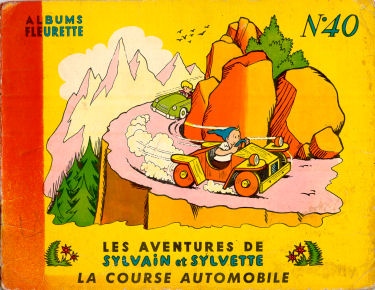
\includegraphics[width=.6\textwidth]{Sylvain+Sylvette_Course.jpg}} 
\newpage           

\item \underline{Résolution du système : }\\

\begin{tabular}{lp{3.5cm}ll}
\multicolumn{4}{l}{
$\begin{cases}
\qquad\dfrac{88}{V_1} -\dfrac{42}{V_2} \!\!\!\!\!\!\!\! &= 1 \\
& \\
\dfrac{106}{V_1} x -\dfrac{24}{V_2} y \!\!\!\!\!\!\!\!&= 1,5  \\
\end{cases}$} \\
& & & \\
\multicolumn{4}{l}{
Le système est linéaire si l'on pose :
       $X=\dfrac{1}{V_1} \text{ et }  Y=\dfrac{1}{V_2}$}\\
& & & \\
\begin{minipage}{4cm}
$\begin{cases}
 \; \; \; 88X - 42Y \!\!\!\!\!\!\!\!&= 1 \\
106X - 24Y\!\!\!\!\!\!\!\! &= 1,5  \\
\end{cases}$ \\
\end{minipage}  &  \multicolumn{1}{|l}{$\begin{array}{l}
                     24\\ -42 \\ 
                  \end{array}$ } & 
                   \begin{minipage}{4cm}       
                         $\begin{cases}
                             \; \; \; 88X - 42Y \!\!\!\!\!\!\!\!&= 1 \\
                            106X - 24Y \!\!\!\!\!\!\!\!&= 1,5  \\
                          \end{cases}$ 
                \end{minipage} &  \multicolumn{1}{|l}{ $\begin{array}{l}
                                        106\\-88\\ 
                                  \end{array}$}\\
& & & \\   
\begin{minipage}{4cm}
$\begin{cases}
 \quad 2112X - 1008Y \!\!\!\!\!\!\!\!&= 24 \\
-4452X - 1008Y \!\!\!\!\!\!\!\!&= -63  \\
\end{cases}$ \\
\end{minipage}  &  & 
                   \begin{minipage}{4cm}       
                         $\begin{cases}
                             \quad 9328X - 4452Y \!\!\!\!\!\!\!\!&= 106 \\
                            -9328X + 2112Y \!\!\!\!\!\!\!\!&= -132  \\
                          \end{cases}$ 
                \end{minipage} &  \\
& & & \\                           
\cline{1-1} \cline{3-3}
\multicolumn{1}{l}{$\qquad \qquad \; \; \; -2340X = -39$} &&
               \multicolumn{1}{l}{$\qquad \qquad \; \; \; -2340Y =-26$}&\\
$\qquad \qquad \qquad \quad \;\; \; X = \dfrac{1}{60}$ && $\qquad \qquad \qquad \quad \;  \; \; Y = \dfrac{1}{90}$& \\
\end{tabular}\\

Il vient : $\dfrac{1}{V_1} = \dfrac{1}{60} $ 
       et  $\dfrac{1}{V_2} = \dfrac{1}{90} $\\


\item \underline{Réponse au problème } :\\

Sylvain roule à 60km/h et les 2 Sylvettes à 90km/h.
  
\end{enumerate} 